\documentclass[10.5pt,scale=1.0,t,aspectratio=169,hyperref={pdfpagelabels=false}]{beamer}


\usepackage{lipsum}
\usepackage{color}
\usepackage{amsfonts}
\usepackage{amsmath,mathtools}
\usepackage{mathrsfs}
\usepackage{array}
\usepackage{algorithm}
\usepackage{hyperref}
\usepackage[spanish,es-nodecimaldot]{babel}
\usepackage[utf8]{inputenc}
\usepackage{graphicx}
\usepackage{multicol}
\usepackage{multirow}
\usepackage{enumitem}
\usepackage[document]{ragged2e}
\usepackage[absolute,overlay]{textpos}
\textblockorigin{0mm}{0mm} 
\usefonttheme[onlymath]{serif}
\usepackage{verbatim}
\usepackage{cite}
\usepackage{multicol}




\newenvironment{conditions}[1][where:]
{#1 \begin{tabular}[t]{>{$}l<{$} @{${}={}$} l}}
	{\end{tabular}\\[\belowdisplayskip]}


\newcolumntype{L}{>{$}l<{$}} % math-mode version of "l" column type


\newcounter{saveenumi}
\newcommand{\seti}{\setcounter{saveenumi}{\value{enumi}}}
\newcommand{\conti}{\setcounter{enumi}{\value{saveenumi}}}

\setbeamertemplate{bibliography item}{\insertbiblabel}


\hypersetup{colorlinks=true,
	linkcolor=blue,
	linktoc=all,				
	citecolor=blue,
	urlcolor=red,
	pdftitle={ELECTRONICA DIGITAL ii},
	pdfauthor={Santiago Rúa Pérez},
	pdfcreator={Santiago Rúa Pérez}}


\definecolor{GreenDark}{rgb}{0.0, 0.60, 0.0}
\definecolor{RedDark}{rgb}{183, 0.0, 0.0}
\definecolor{BlueDark}{rgb}{0.0, 0.0, 167}
\definecolor{BlueLight}{rgb}{0.2, 0.451, 0.517}


\graphicspath{{imag/}}

\newcommand{\Ho}{$H_{0}$}
\newcommand{\Ha}{$H_{a}$}
\newcommand{\Nota}{{\bf Nota: }}
\newcolumntype{P}[1]{>{\centering\arraybackslash}p{#1}}
\newcolumntype{M}[1]{>{\centering\arraybackslash}m{#1}}

\newcommand{\less}{<}
\newcommand{\greater}{>}


\setlength{\parindent}{1em}
\setlength{\parskip}{.6em}
\renewcommand{\baselinestretch}{.9}

%%%%    C environment    ---------------- %%%%%%%%%%%%%%%.
\usepackage{listings}
\usepackage{xcolor}
\definecolor{mGreen}{rgb}{0,0.6,0}
\definecolor{mGray}{rgb}{0.5,0.5,0.5}
\definecolor{mPurple}{rgb}{0.58,0,0.82}
\definecolor{backgroundColour}{rgb}{0.95,0.95,0.92}

\lstdefinestyle{CStyle}{
	backgroundcolor=\color{backgroundColour},   
	commentstyle=\color{mGreen},
	keywordstyle=\color{magenta},
	numberstyle=\tiny\color{mGray},
	stringstyle=\color{mPurple},
	basicstyle=\scriptsize,
	breakatwhitespace=false,         
	breaklines=true,                 
	captionpos=b,                    
	keepspaces=true,                 
	numbers=left,                    
	numbersep=5pt,                  
	showspaces=false,                
	showstringspaces=false,
	showtabs=false,                  
	tabsize=2,
	language=C
}
%%--------------------------------------------------------------------------


\title{Electrónica Digital II}   
\author{Santiago Rúa Pérez, PhD.} 
\date{\today} 

\setlength{\TPHorizModule}{\textwidth}
\setlength{\TPVertModule}{\textwidth}

\newcommand{\btVFill}{\vskip0pt plus 1filll}


\setbeamertemplate{sidebar right}{}
\setbeamertemplate{footline}
{
	\leavevmode%
	\hbox{%
		\begin{beamercolorbox}[wd=.333333\paperwidth,ht=2.25ex,dp=1ex,center]{author in head/foot}%
			\usebeamerfont{author in head/foot}\insertshortauthor
		\end{beamercolorbox}%
		\begin{beamercolorbox}[wd=.333333\paperwidth,ht=2.25ex,dp=1ex,center]{title in head/foot}%
			\usebeamerfont{title in head/foot}\insertshorttitle
	\end{beamercolorbox}}%
	\vskip0pt%
}
\makeatother

\begin{document}
	%%%%%%%%%%%%%%%%%% FRAME %%%%%%%%%%%%%%%%%%%%%%%%%%
	\begin{frame}
		\titlepage
	\end{frame}
	%%%%%%%%%%%%%%%%% FRAME START %%%%%%%%%%%%%%%%%%%%%%%%%%
	\frame{
		%\frametitle{}
		\begin{center}
			\LARGE \textcolor{blue}{INTERRUPCIONES}
		\end{center}
		
	}
	
	%%%%%%%%%%%%%%%%% FRAME %%%%%%%%%%%%%%%%%%%%%%%%%%

%%%%%%%%%%%%%%%%% FRAME %%%%%%%%%%%%%%%%%%%%%%%%%%
\begin{frame}
	\frametitle{Objetivos}
	\begin{itemize}
		\item Entender los conceptos de excepciones e interrupciones
		\begin{itemize}
			\item Entrando en el manejo de una excepción.
			\item Saliendo del manejo de una excepción.
		\end{itemize}
		\item Cortex-M4 interrupciones.
		\item Análisis de tiempos
		\item Diseño de programas con interrupciones.
		\item Fuentes
		\begin{itemize}
			\item \href{https://developer.arm.com/documentation/dui0553/latest/}{Cortex M4 Device Generic User Guide - DUI0553}
			\item \href{https://developer.arm.com/documentation/ddi0439/b/}{Cortex M4 Technical Reference Manual - DDI0439B}
		\end{itemize}
	\end{itemize}
\end{frame}
%%%%%%%%%%%%%%%%% FRAME %%%%%%%%%%%%%%%%%%%%%%%%%%
\begin{frame}
	\frametitle{Ejemplo de sistema con interrupción}
	\begin{figure}
		\centering
		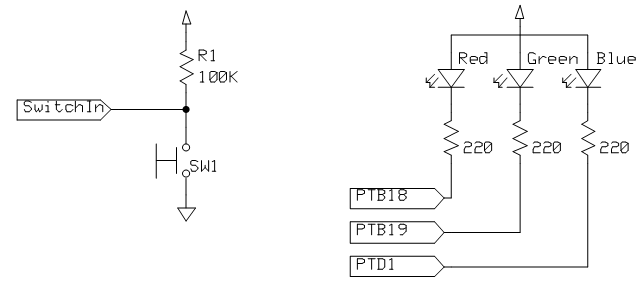
\includegraphics[scale=0.6]{01_EjemploInterrupcion}
	\end{figure}
	\begin{itemize}
		\item Meta: cambiar el color del led RGB cuando se presiona el suiche.
		\item Explicar en detalle la interfaz entre el suiche y el módulo LED.
		\item Necesidad de adicionar suiche externo. 
	\end{itemize}
\end{frame}
%%%%%%%%%%%%%%%%% FRAME %%%%%%%%%%%%%%%%%%%%%%%%%%
\begin{frame}
	\frametitle{Cómo detectar cuando se presiona el suiche?}
	\begin{itemize}
		\item Haciendo polling - a través de software.
		\begin{itemize}
			\item Lento - se necesita explícitamente estar monitoreando el suiche y preguntar por el mismo.
			\item Desperdicio de tiempo de la CPU - entre más rápido necesitemos una respuesta, mas seguido necesitamos estar chequeando. 
			\item Escalabilidad mala - difícil construir sistema con muchas actividades que puedan responder de forma ágil. Dependerá de otros procesos.
		\end{itemize}
		\item Interrupciones - Uso especial de hardware dentro del MCU para detectar eventos, corre un código específico (interrupt service routine - ISR)
		\begin{itemize}
			\item Eficiente - el código solo se ejecuta cuando es necesario.
			\item Rápido - mecanismo de hardware.
			\item Escalabilidad buena
			\begin{itemize}
				\item El tiempo de respuesta del ISR no depende de otros procesos. 
				\item Los módulos pueden desarrollarse de forma independiente. 
			\end{itemize}
		\end{itemize}
	\end{itemize}
\end{frame}
%%%%%%%%%%%%%%%%% FRAME %%%%%%%%%%%%%%%%%%%%%%%%%%
\begin{frame}
	\frametitle{Secuencia de la interrupción}
	\begin{columns}
		\column{0.5\linewidth}
		\begin{itemize}
			\item El código principal esta corriendo.
			\item Ocurre algo que dispara la interrupción.
			\item El procesador hace un procesamiento de manejo del hardware.
			\item El procesador ejecuta ISR.
			\item El procesador hace manejo de hardware.
			\item El procesador continua con la ejecución del programa. 
		\end{itemize}
	
		\column{0.5\linewidth}
		\begin{figure}
			\centering
			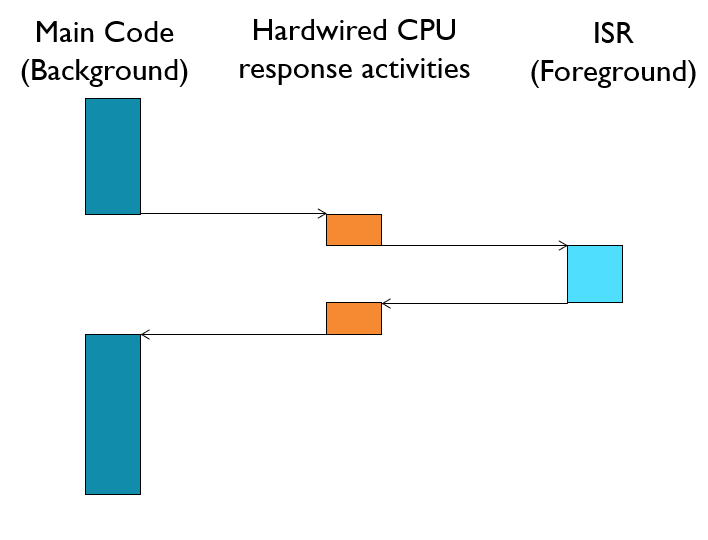
\includegraphics[scale=0.4]{02_EjecucionInterrupcion}
		\end{figure}
	\end{columns}
\end{frame}
%%%%%%%%%%%%%%%%% FRAME %%%%%%%%%%%%%%%%%%%%%%%%%%
\begin{frame}
	\frametitle{Secuencia de la interrupción}
	\begin{itemize}
		\item Rutina asincronica disparada por hardware.
		\begin{itemize}
			\item Disparado por una señal de hardware.
			\item Asincrónico - puede pasar en cualquier momento del programa. 
			\item Rutina por software - Servicio de rutina corre como respuesta a la interrupción. 
		\end{itemize}
		\item Mecanismo fundamental de los microcontroladores.
		\begin{itemize}
			\item Genera un procedimiento eficiente basado en evento en vez de polling
			\item Genera una respuesta rápida sin importar el estado del programa.
			\item Permite muchos hilos en sistemas embebidos sin la necesidad de sistemas operativos. 
		\end{itemize}
	\end{itemize}
\end{frame}
%%%%%%%%%%%%%%%%% FRAME %%%%%%%%%%%%%%%%%%%%%%%%%%
\begin{frame}
	\frametitle{Ejemplo de uso}
	\begin{figure}
		\centering
		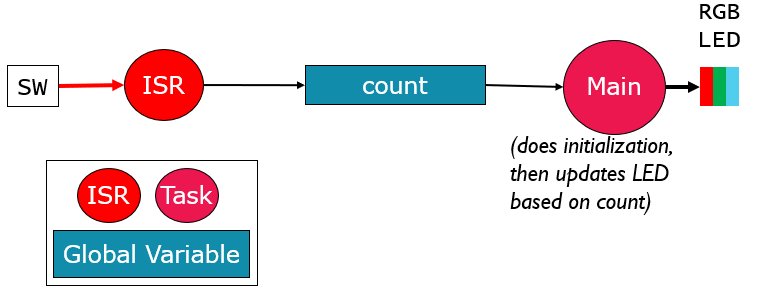
\includegraphics[scale=0.4]{03_EjemploInt}
	\end{figure}
	\begin{itemize}
		\item Req1: cuando el suiche 1 es presionado, ISR incrementará un contador.
		\item Req2: el código principal prende los leds de acuerdo al valor del contador (Azul: 4, Verde:2, Rojo:1).
		\item Req3: ISR se ejecuta de acuerdo a la interrupción. 
	\end{itemize}
\end{frame}
%%%%%%%%%%%%%%%%% FRAME %%%%%%%%%%%%%%%%%%%%%%%%%%
\begin{frame}
	\frametitle{Entrando al administrador de la excepción}
	\begin{itemize}
		\item Terminar la instrucción actual (excepto las largas).
		\item Guarda todo el contexto de los registros en el stack actual.
		\item Cambiar el modo de operación.
		\item Carga en el PC el administrador de la excepción.
		\item Carga registros LR y IPSR.
		\item Inicia ejecución de la interrupción. 
	\end{itemize}
	Usualmente le toma al procesador 16 ciclos. 
\end{frame}
%%%%%%%%%%%%%%%%% FRAME %%%%%%%%%%%%%%%%%%%%%%%%%%
\begin{frame}
	\frametitle{Saliendo de la interrupción}
	\begin{itemize}
		\item Ejecuta el proceso de la interrupción.
		\item Selecciona el stack de retorno, restaura contexto.
		\item Vuelve a la ejecución del programa normal. 
	\end{itemize}
\end{frame}
%%%%%%%%%%%%%%%%% FRAME %%%%%%%%%%%%%%%%%%%%%%%%%%
\begin{frame}
	\frametitle{Interrupciones del microcontrolador Cortex M4}
	\begin{itemize}
		\item Tipos de interrupciones.
		\begin{itemize}
			\item Interrupciones por hardware.
			\begin{itemize}
				\item \textbf{Asíncronas}: no estan relacionadas con lo que el procesador está ejecutando. 
				\item Ejemplo: se termina la interrupción, un caracter es recibido en el puerto serial, el ADC termina la conversión. 
			\end{itemize}
			\item Excepciones, fallas o interrupciones por software.
			\begin{itemize}
				\item \textbf{Síncronas}: son el resultado de la ejecución específica de un código.
				\item Ejemplos: instrucciones sin definir, overflow ocurre en la ejecución de una instrucción.
			\end{itemize}
			\item La mayoría de interrupciones se pueden habilitar o deshabilitar cuando se necesite.  
		\end{itemize}
		\item Rutina de servicio de interrupcción.
		\begin{itemize}
			\item Subrutina que el procesador se ve obligado a realizar para responder a un evento específico dentro del procesador.
			\item Despues de que se complete el ISR, MCU vuelve a donde se estaba ejecutando. 
		\end{itemize}
	\end{itemize}
\end{frame}
%%%%%%%%%%%%%%%%% FRAME %%%%%%%%%%%%%%%%%%%%%%%%%%
\begin{frame}
	\frametitle{Ejemplo de uso}
	\begin{figure}
		\centering
		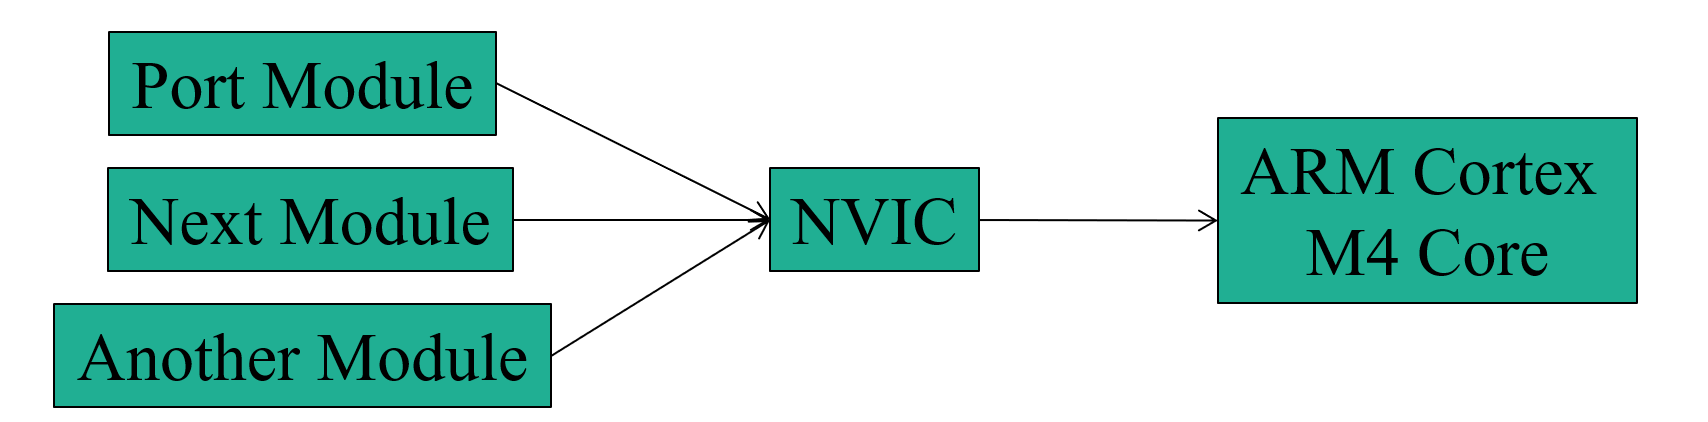
\includegraphics[scale=0.35]{04_NVIC}
	\end{figure}
	\begin{itemize}
		\item NVIC (\textit{Nested Vector Interrupt Controller}) maneja y prioriza las interrupciones externas del MCU. 
		\item Las interrupciones son un tipo de excepciones.
		\item Modos
		\begin{itemize}
			\item Thread Mode: se entra cuando se genera un reset.
			\item Handler mode: entra para ejecutar una excepción.
		\end{itemize}
		\item Nivel de privilegios.
		\item Stack pointers.
		\begin{itemize}
			\item Main Stack Pointer, MSP
			\item Process Stack Pointer, PSP
		\end{itemize}
		\item Estados de excepción: inactivo, pendiente, activo.
	\end{itemize}
\end{frame}
%%%%%%%%%%%%%%%%% FRAME %%%%%%%%%%%%%%%%%%%%%%%%%%
\begin{frame}
	\frametitle{Algunas fuente de interrupciones}
	\begin{table}
		\centering
		\begin{tabular}{ccccc}
			\hline
			\textbf{Address} & \textbf{Vector} & \textbf{IRQ} & \textbf{Source} & \textbf{Description} \\
			\hline
			0x0000\_0004 & 1 & & ARM Core & Initial program counter \\
			0x0000\_0008 & 2 & & ARM Core & Non-maskable interrupt \\
			0x0000\_0040-80 & 16-32 & 0-16 & DMA controller & Transfer complete or error \\
			0x0000\_00A0-A4 & 40-41 & 24-25 & I2C & Status and error \\
			0x0000\_00A8-AC & 42-43 & 26-27 & SPI & Status and error \\
			0x0000\_00BC-D8 & 47-54 & 31-38 & UART & Status and error \\
			0x0000\_012C & 75 & 59 & Port Control Module & Port A \\
			0x0000\_0130 & 76 & 60 & Port Control Module & Port B \\
			0x0000\_0134 & 77 & 61 & Port Control Module & Port C \\
			0x0000\_0138 & 78 & 62 & Port Control Module & Port D \\
			0x0000\_013C & 79 & 63 & Port Control Module & Port E \\
			\hline
		\end{tabular}
	\end{table}
	Hasta 85 vectores diferentes del procesador, 16 del procesador principal. Table 3-5 reference manual. 
\end{frame}
%%%%%%%%%%%%%%%%% FRAME %%%%%%%%%%%%%%%%%%%%%%%%%%
\begin{frame}
	\frametitle{NVIC registros y estados}
	\begin{figure}
		\centering
		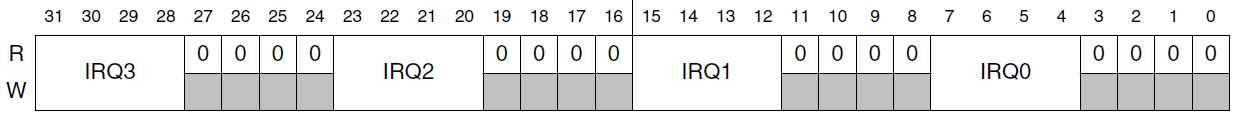
\includegraphics[scale=0.6]{05_IPR0}
	\end{figure}
	\begin{itemize}
		\item Prioridad - permite al programa priorizar la respuesta si ocurren dos interrupciones. 
		\item IPR0-59 registros: 4 bits por interrupcion, cuantro fuentes de interrupción por registro. 
		\item La prioridad 0 es la de mayor atención. 
		\item CMSIS: NVIC\_SetPriority(IRQnum,priority)
		\item Enable: permite habilitar las interrupciones.
		\begin{itemize}
			\item Se accesan con dos registros: Set enable con NVIC\_ISER, clear enable con NVIC\_ICER
			\item CMSIS: NVIC\_EnableIRQ(IRQnum), NVIC\_DisableIRQ(IRQnum)
		\end{itemize}
		\item Pending: la interrupción se dio, pero no ha sido atendida.
		\begin{itemize}
			\item CMSIS:  NVIC\_SetPendingIRQ(IRQnum), NVIC\_ClearPendingIRQ(IRQnum)
		\end{itemize}
	\end{itemize}
\end{frame}
%%%%%%%%%%%%%%%%% FRAME %%%%%%%%%%%%%%%%%%%%%%%%%%
\begin{frame}
	\frametitle{Excepciones del procesador}
	\begin{itemize}
		\item Similar a deshabilitar interrupciones globales en la MCU.
		\item PRIMASK - registro de mascara de excepción
		\begin{itemize}
			\item Solo utiliza el bit cero.
			\item Ponerlo en 1 evita la activación de cualquier interrupción.
			\item Ponerlo en 0 permite la activación de todas las excepciones. 
			\item Ayuda a prevenir borrado de datos o condiciones extrañas de comportamiento.
		\end{itemize}
		\item CMSIS-CORE API
		\begin{itemize}
			\item void \_\_enable\_irq() - clears PM flag
			\item void \_\_disable\_irq() - sets PM flag
			\item uint32\_t \_\_get\_PRIMASK() - returns value of PRIMASK
			\item void \_\_set\_PRIMASK(uint32\_t x) - sets PRIMASK to x 
		\end{itemize}
	\end{itemize}
\end{frame}
%%%%%%%%%%%%%%%%% FRAME %%%%%%%%%%%%%%%%%%%%%%%%%%
\begin{frame}
	\frametitle{Priorización}
	\begin{itemize}
		\item Las excepciones son priorizadas para responder en orden de acuerdo a la solicitud dada (número pequeño = mayor la prioridad)
		\item Algunas prioridades están fijas.
		\begin{itemize}
			\item Reset: -3, mayor prioridad.
			\item NMI: -2
			\item Hard fault: -1
		\end{itemize}
		\item Las prioridades de los periféricos son ajustables. 
		\begin{itemize}
			\item Los valores son almacenados en el registro de prioridad de la interrupción IPR
			\item Un valor por encima de cero. 
		\end{itemize}
		\item Solicitud simultanea de excepciones? Se atiende la de menor número.
		\item Una nueva excepción se requiere mientras se está atendiendo otra interrupción?
		\begin{itemize}
			\item La nueva tiene mayor prioridad? Se atiende la nueva excepción. 
			\item Es menor? entonces se pone en estado pendiente. Termina la ejecución de la actual y se atiende la nueva. 
		\end{itemize}
	\end{itemize}
\end{frame}
%%%%%%%%%%%%%%%%% FRAME %%%%%%%%%%%%%%%%%%%%%%%%%%
\begin{frame}
	\frametitle{Ejemplo}
	\begin{figure}
		\centering
		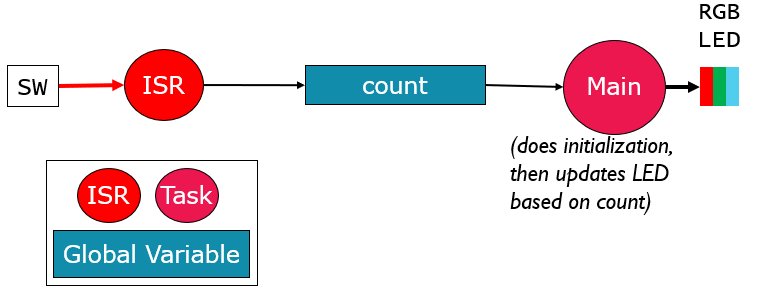
\includegraphics[scale=0.4]{03_EjemploInt}
	\end{figure}
	\begin{itemize}
		\item Req1: cuando el suiche 1 es presionado, ISR incrementará un contador.
		\item Req2: el código principal prende los leds de acuerdo al valor del contador (Azul: 3, Verde:2, Rojo:1).
		\item Req3: ISR se ejecuta su linea de acuerdo a la interrupción. 
	\end{itemize}
\end{frame}
%%%%%%%%%%%%%%%%% FRAME %%%%%%%%%%%%%%%%%%%%%%%%%%
\begin{frame}
	\frametitle{Construyendo el programa}
	\begin{itemize}
		\item Primero haga el paso al paso del programa en pequeños pasos.
		\begin{itemize}
			\item Programa principal:
			\begin{itemize}
				\item Inicializar el sistema.
				\item Inicializar suiche
				\item Inicializar el led.
				\item Inicializar las interrupciones.
				\item Luego repita
				\item Actualizar el led basado en el contador. 
			\end{itemize}
			\item Atención a la interrupción
			\begin{itemize}
				\item Actualizar el contador. 
			\end{itemize}
		\end{itemize}
		\item Determinar que variable se va a compartir entre el programa principal y la atención a la interrupción.
		\begin{itemize}
			\item A través de variables globales se comunican el programa principal y la interrupción.
			\item Siempre declare las variables compartidas como volatile.
			\item Asegure que el acceso de la variable es atómico. 
		\end{itemize}
	\end{itemize}
\end{frame}
%%%%%%%%%%%%%%%%% FRAME %%%%%%%%%%%%%%%%%%%%%%%%%%
\begin{frame}
	\frametitle{Panorama general}
	\begin{itemize}
		\item main
		\begin{itemize}
			\item Nivel más arriba de ejecución.
		\end{itemize}
		\item suiches
		\begin{itemize}
			\item \#defines para las conexiones del suiche
			\item declaración de la variable contador.
			\item código para inicializar suiche e interrupción.
			\item ISR para el suiche.
		\end{itemize}
		\item Leds
		\begin{itemize}
			\item \#define para las conexiones del led.
			\item Código para inicializar el Led.
		\end{itemize}
		\item debug\_signals
		\begin{itemize}
			\item \#define para la señal de debug.
			\item Código para inicializar el debug.
		\end{itemize}
	\end{itemize}
\end{frame}
%%%%%%%%%%%%%%%%% FRAME %%%%%%%%%%%%%%%%%%%%%%%%%%
\begin{frame}
	\frametitle{Port module}
	\begin{figure}
		\centering
		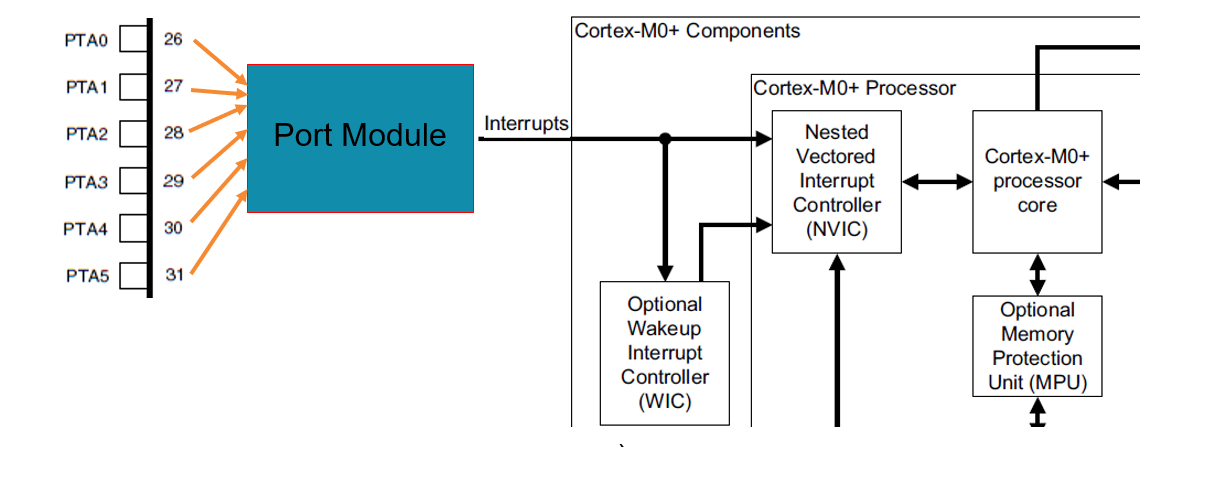
\includegraphics[scale=0.5]{06_PortInterrupt}
	\end{figure}
	\begin{itemize}
		\item Los puertos estan conectado al NVIC.
		\item Registros relevantes
		\begin{itemize}
			\item PCR
			\begin{itemize}
				\item Cada registro corresponde a la entrada de un pin.
			\end{itemize}
			\item ISFR
			\begin{itemize}
				\item Cada bit corresponde a una entrada.
				\item El bit es uno si ha sido detectada una interrupción. 
			\end{itemize}
		\end{itemize}
	\end{itemize}
\end{frame}
%%%%%%%%%%%%%%%%% FRAME %%%%%%%%%%%%%%%%%%%%%%%%%%
\begin{frame}
	\frametitle{Pin Control Register}
	\begin{figure}
		\centering
		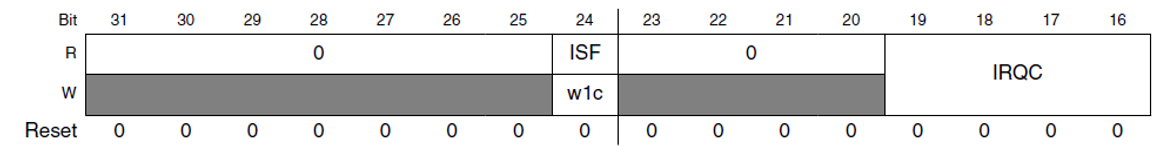
\includegraphics[scale=0.6]{07_PCR}
	\end{figure}
	\begin{columns}
		\column{0.5\linewidth}
		\begin{itemize}
			\item ISF indica si se ha detectado una interrupción. Es lo mismo que acceder al ISFR.
			\item IRQC define el comportamiento externo
			\item También puede trabajar con acceso directo a memoria.
		\end{itemize}
		
		\column{0.5\linewidth}
		\begin{table}
			\begin{tabular}{cc}
				\hline 
				\textbf{IRQC} & \textbf{Configuración} \\
				\hline
				0000 & Interrupción deshabilitada \\
				... & DMA \\
				1000 & Interrupción cuando es cero \\
				1001 & Interrupción en flanco de subida \\
				1010 & Interrupción en flanco de bajada \\
				1011 & Interrupción en los dos casos\\
				1100 & Interrupción cuando es uno \\
				\hline
			\end{tabular}
		\end{table}
	\end{columns}
\end{frame}
%%%%%%%%%%%%%%%%% FRAME %%%%%%%%%%%%%%%%%%%%%%%%%%
\begin{frame}[fragile]
	\frametitle{Inicialización de la interrupción}
	\begin{lstlisting}[style=CStyle]
void init_switch(void){
	//Clock activation PTA
	SIM->SCGC5 |= SIM_SCGC5_PORTA_MASK; 
	
	// Port as GPIO and interrupt in falling edge
	PORTA->PCR[SW1] = PORT_PCR_MUX(1) | PORT_PCR_IRQC(0x0A);
	
	// GPIO as input (PTA4)
	PTA->PDDR &= ~MASK(SW1);
	
	/* Enable Interrupts */
	NVIC_SetPriority(PORTA_IRQn, 2);
	NVIC_ClearPendingIRQ(PORTA_IRQn);
	NVIC_EnableIRQ(PORTA_IRQn);
	
}
	\end{lstlisting}
\end{frame}
%%%%%%%%%%%%%%%%% FRAME %%%%%%%%%%%%%%%%%%%%%%%%%%
\begin{frame}[fragile]
	\frametitle{Atención a interrupción}
	Rutina de servicio de atención a interrupción. 
	\begin{lstlisting}[style=CStyle]
void PORTA_IRQHandler(void) {
	if ((PORTA->ISFR & MASK(SW1))) {
		band=1;
	}
	// clear status flags
	PORTA->ISFR = 0xffffffff;
}
	\end{lstlisting}

Programa principal
\begin{lstlisting}[style=CStyle]
int main(void) {
	__disable_irq();            /* disable all IRQs */
	init_rgb();
	init_switch();
	__enable_irq();             /* global enable IRQs */
	while(1) {
		RGB_task();
		__wfi();
	}
	return 0 ;
}
\end{lstlisting}
\end{frame}
%%%%%%%%%%%%%%%%% FRAME %%%%%%%%%%%%%%%%%%%%%%%%%%
\begin{frame}[fragile]
	\frametitle{Tarea RGB}
	Máquina de estados para la tarea RGB
	\begin{lstlisting}[style=CStyle]
void RGB_task(void){
	static enum {L_RED,L_GREEN,L_BLUE} next_state=L_RED;
	if(band==1){
		switch(next_state){
			case L_RED:
				Control_RGB_LEDs(1,0,0);
				next_state=L_GREEN;
				break;
			case L_GREEN:
				Control_RGB_LEDs(0,1,0);
				next_state=L_BLUE;
				break;
			case L_BLUE:
				Control_RGB_LEDs(0,0,1);
				next_state=L_RED;
				break;
		}
		band = 0;
	}
}
	\end{lstlisting}
\end{frame}
%%%%%%%%%%%%%%%%% FRAME %%%%%%%%%%%%%%%%%%%%%%%%%%
\begin{frame}
	\frametitle{Características del ISR}
	\begin{itemize}
		\item No hay argumentos o valores de retorno en la función - void es el unico tipo de datos válido.
		\item Mantenerlo corto y simple
		\begin{itemize}
			\item Más fácil de hacer debug.
			\item Mejora el tiempo de respuesta del sistema.
		\end{itemize}
		\item Nombre la función del ISR de acuerdo al sistema de excepcion del CMSIS-CORE 
		\item Lea el registro con la bandera de status para determinar quien genero la interrupción.
		\item Limpie la bandera escribiendo unos en el ISFR. 
	\end{itemize}
\end{frame}
%%%%%%%%%%%%%%%%% FRAME %%%%%%%%%%%%%%%%%%%%%%%%%%
\begin{frame}
	\frametitle{Datos volatiles}
	\begin{itemize}
		\item Los compiladores asumen que las variables en memoria no cambian espontáneamente y optimizan código con base en esto.
		\begin{itemize}
			\item No vuelven a cargar desde memoria si la función actual no la ha cambiado. 
			\item Carga la variable desde memoria a los registros (acceso más rápido).
			\item Escribe de nuevo en memoria cuando el procedimiento a terminado o cuando se queda sin registros que compilar. 
		\end{itemize}
		\item La optimización puede fallar.
		\item Variables que pueden fallar:
		\begin{itemize}
			\item Registros de periféricos mapeados en memoria - el registro cambia por si mismo.
			\item Variables globales modificas por ISR - ISR cambia la variable.
			\item Variables globales en una aplicación multihilos. 
		\end{itemize}
	\end{itemize}
\end{frame}
%%%%%%%%%%%%%%%%% FRAME %%%%%%%%%%%%%%%%%%%%%%%%%%
\begin{frame}
	\frametitle{Datos compartidos no anatómicos}
	Algunos datos o objetos le toman múltiples operaciones para ser modificados. 
	\begin{columns}
		\column{0.5\linewidth}
		\begin{itemize}
			\item Se desea mantener un manejo del tiempo.
			\item Se utiliza una interrupción de un segundo. 1Hz.
			\item Sistema
			\begin{itemize}
				\item La estructura TimerVal lleva el conteo.
				\item La estructura se actual dentro de la rutina ISR.
			\end{itemize}
		\end{itemize}
	
		\column{0.5\linewidth}
		\begin{figure}
			\centering
			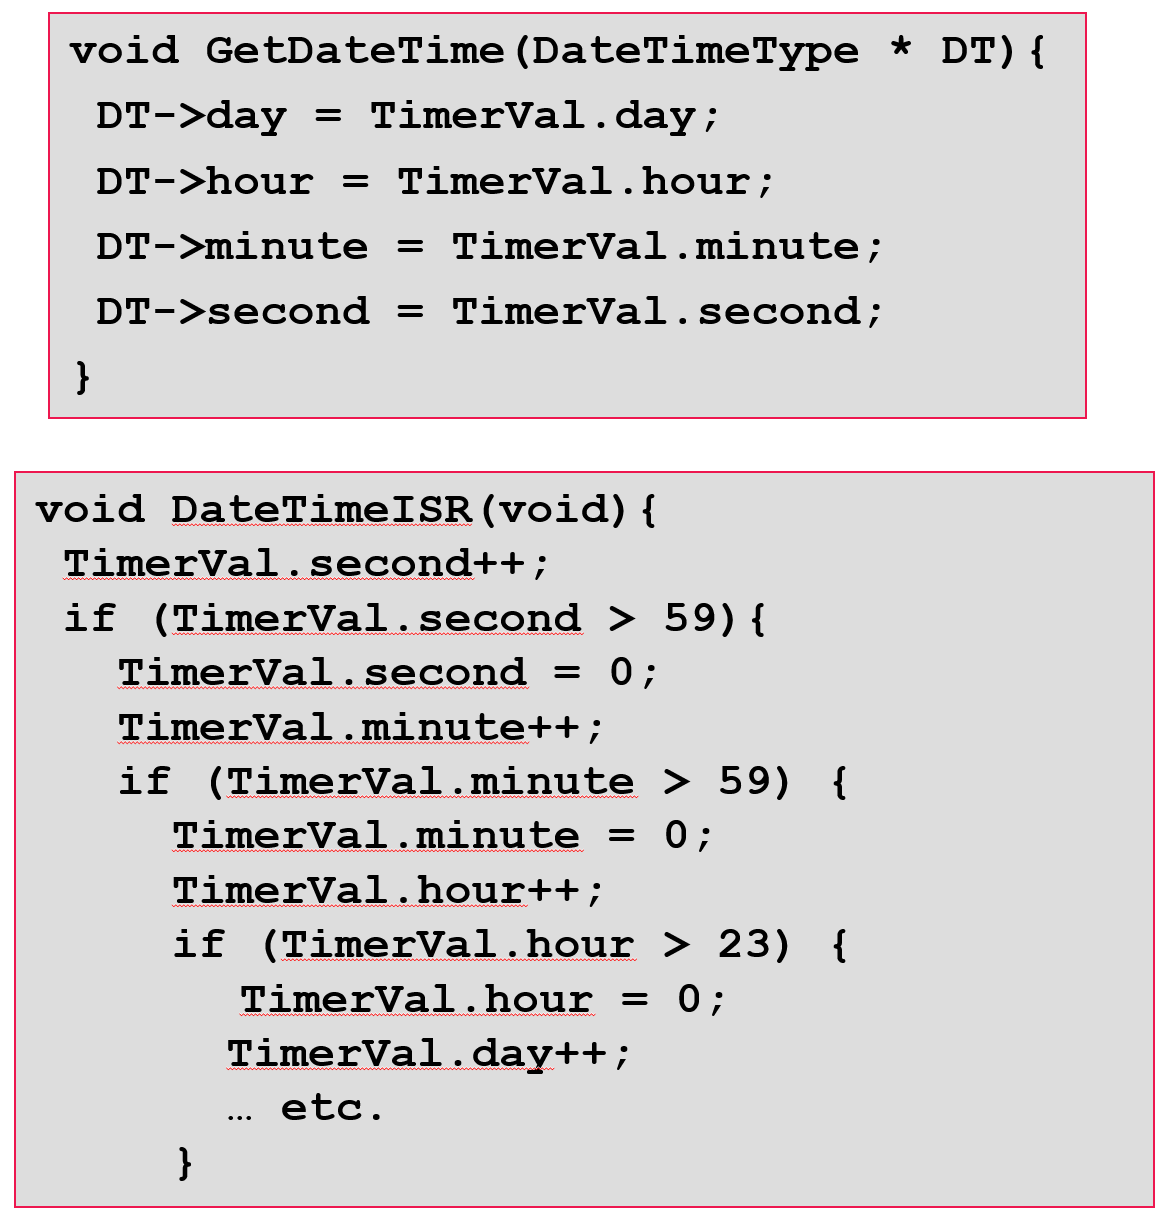
\includegraphics[scale=0.3]{08_Atomic}
		\end{figure}
	\end{columns}
\end{frame}
%%%%%%%%%%%%%%%%% FRAME %%%%%%%%%%%%%%%%%%%%%%%%%%
\begin{frame}
	\frametitle{Datos compartidos no anatómicos - Problema?}
	\begin{itemize}
		\item Problema
		\begin{itemize}
			\item Una interrupción en el momento inadecuado puede ocasionar una falla en la actualización de DT
		\end{itemize}
		\item Caso de falla
		\begin{itemize}
			\item TimerVal es \{10, 23, 59, 59\} (10th day, 23:59:59)
			\item El código principal llama a la tarea GetDateTime(), el cual comienza la actualización de los datos. DT: day = 10, hour = 23
			\item Una interrupción por timer ocurre, se actualiza TimerVal a \{11, 0, 0, 0\}
			\item GetDateTime() retoma la ejecución y copia el restos de los campos de DT: minute = 0, second = 0
			\item DT ahora vale {10, 23, 0, 0}
			\item El sistema piensa que salto una hora antes. 
		\end{itemize}
		\item Problema fundamental - \textbf{Condición de carrera}
		\begin{itemize}
			\item Preemption le posibilita al ISR tomar el control y posiblemente reescribir data.
			\item Se debe asegurar acceso atómico (indivisible) al objeto. Por ejemplo si el procesador es de 32 bits, tengo variables mas grandes?
		\end{itemize}
	\end{itemize}
\end{frame}
%%%%%%%%%%%%%%%%% FRAME %%%%%%%%%%%%%%%%%%%%%%%%%%
\begin{frame}
	\frametitle{Definiciones}
	\begin{itemize}
		\item \textbf{Condición de carrera}: Comportamiento anómalo debido a una dependencia crítica inesperada del momento relativo de los eventos. El resultado del código de ejemplo depende del tiempo relativo de las operaciones de lectura y escritura.
		\item \textbf{Sección crítica}: Una sección de código que crea una posible condición de carrera. La sección de código solo puede ser ejecutada por un proceso a la vez. Se requiere algún mecanismo de sincronización en la entrada y salida de la sección crítica para asegurar el uso exclusivo.
	\end{itemize}
\end{frame}
%%%%%%%%%%%%%%%%% FRAME %%%%%%%%%%%%%%%%%%%%%%%%%%
\begin{frame}
	\frametitle{Solución - Deshabilitar momentáneamente Preemption}
	\begin{columns}
		\column{0.7\linewidth}
		\begin{itemize}
			\item Prevenir preemption dentro de una sección crítica del código.
			\item Si ISR puede escribir a una variable compartida, entonces se debe deshabilitar esa sección.
			\begin{itemize}
				\item Almacenar el estado actual de la interrupción
				\item deshabilite interrupciones hasta que actualice las variables compartidas.
			\end{itemize}
			\item Restaure el estado anterior.
			\item Use el CMSIS-CORE para guardar, almacenar, y restaurar las interrupciones. 
			\item Evite si es posible la desactivación de las interrupciones si retrasa la respuesta a todas las demás solicitudes de procesamiento
			\item Que sea el tiempo mas corto posible. 
		\end{itemize}
		
		\column{0.3\linewidth}
		\begin{figure}
			\centering
			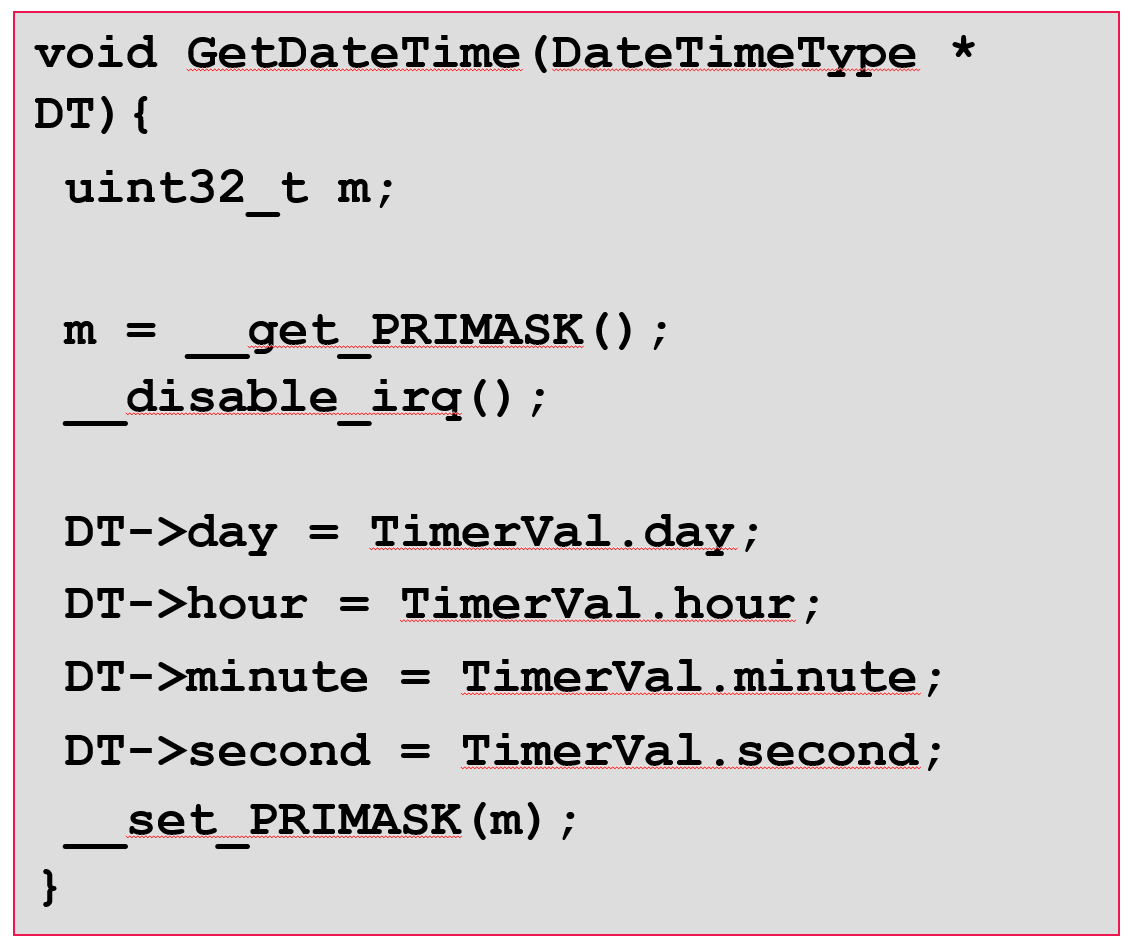
\includegraphics[scale=0.25]{09_DisablePreemption}
		\end{figure}
	\end{columns}
\end{frame}
%%%%%%%%%%%%%%%%% FRAME %%%%%%%%%%%%%%%%%%%%%%%%%%
\begin{frame}
	\frametitle{Laboratorio 3 (10\%)}
	\begin{itemize}
		\item Realice un juego de simon dice con cuatro pulsadores y cuatro leds externos. El objetivo es que el sistema genere una secuencia de pulsaciones de los led para que el usuario siga en el mismo orden. Utilice interrupciones para los cuatro pulsadores externos. A continuación les dejo un enlace
		
		\href{https://www.youtube.com/watch?v=PK7zc28IGPc}{Video de simon dice}
	\end{itemize}
\end{frame}
%%%%%%%%%%%%%%%%% FRAME %%%%%%%%%%%%%%%%%%%%%%%%%%
\frame{
\begin{center}
	\LARGE \textcolor{blue}{INTERRUPCIONES}
\end{center}

\begin{center}
	\LARGE \textcolor{blue}{GRACIAS}
\end{center}
}

%%%%%%%%%%%%%%%%%%%%%%%%%%%%%%%%%%%%%%%%%%%%%%%%%%%%%%%%%%%%%%%%%%%%%%%%%%%%%%%%%%%%%%%%%%%%%%%%%%%%%%%%%%%%%



\end{document}

